\chapter{Senzory a akční plány}

\section{Motivace}
V této kapitole se již přesouváme od hry samotné ke způsobu, jak na daný stav hry nahlížet chytřeji a také, jak na něj chytřeji reagovat. 
Na nejnižší úrovni dostávají agenti od prostředí stav, který obsahuje seznamy všech vesmírných objektů a agenti na něj mají reagovat nějakou elementární akcí.
Bylo by proto dobré vymyslet princip, jak z obsáhlých a detailních informací nízké úrovně získávat menší objemy zajímavějších informací vyšší úrovně. 
A podobně by se nám mohlo hodit místo elementárních akcí nízké úrovně, vymyslet princip jak volit akce tak, aby vedly k akcím vyšší úrovně.
A právě tyto abstrakce realizujeme pomocí senzorů a akčních plánů.
\section{Senzor}

Senzorem nazveme metodu, která nám z kompletního stavu reprezentovaného seznamem vesmírných objektů extrahuje nějakou užitečnou informaci, která není ve stavu explicitně zadána.
Informace získané z těchto senzorů, respektive senzorických metod, můžeme využít v rozhodovacím problému vybrání akcí.
Většina senzorických metod využívá simulování hry. Na základě současného rozpoložení vesmírných objektů ve stavu se v rámci simulace pokračuje v jejich pohybu, tak jak by se pohybovaly, pokud by žádný z hráčů neprováděl žádné akce.
A na základě toho, co se stane v nejbližších krocích simulace, můžeme zjistit konkrétní informace, které platí o současném stavu hry.
V simulaci žádný z hráčů neprovádí žádné akce, kromě těch, na jejichž dopad se v dané simulaci dotazujeme.
Všechny simulace probíhají omezený počet kroků. Tento počet kroků je roven konstantě \emph{\uppercase{Impact\_radius}}. Pro tuto hodnotu se mi ukázal být vhodný počet 25.
Je to dostatečně vysoká hodnota, aby senzory včas zaznamenaly potřebné informace a zároveň je dostatečně nízká, aby senzorické metody nebyly výpočetně zbytečně náročné.



\subsection{Příklady senzorů}
\begin{itemize}
    \item První sražený neutrální asteroid - Zde se simuluje pohyb vesmírné lodi, střel a neutrálních asteroidů. 
    V případě, že v simulaci dojde k srážce vesmírné lodi a neutrálního asteroidu, vrací tento senzor daný asteroid a počet kroků, po kterém došlo ke srážce.
    Berou se zde v úvahu i vlastní střely. Pokud dojde k sestřelení asteroidu střelou, jsou jak asteroid, tak i střela odstraněny z následné simulace.
    \item První sražený nepřátelský asteroid - Jde o téměř identický senzor, jen s rozdílem, že se nesoustředí na asteroidy neutrální, ale na asteroidy nepřátelské.
    \item Asteroid zasáhne nepřátelskou loď - Zde se simuluje pouze pohyb konkrétního asteroidu a nepřátelské lodí. 
    Opět je zde nastaven daný limit na počet simulovaných kroků. 
    Senzor vrací informaci zda, a v kolika krocích se střetl s nepřátelskou lodí.
    V simulaci nepřátelská loď neprovádí žádné reakce.
    \item Střela zasáhne konkrétní asteroid - Jde o simulaci podobnou předchozí. Simuluje se pohyb konkrétního asteroidu a konkrétní střely.
    \item Střela zasáhne libovolný asteroid - Simuluje se pohyb konkrétní střely a všech neutrálních a nepřátelských asteroidů.
        Tato senzorická metoda vrací zda střela zasáhla sestřelila asteroid, daný asteroid a počet kroků, po kterém střela sestřelila asteroid.
    \item Vzdálenost dvou bodů - Vrátí vzdálenost vyjádřenou v Euklidovské metrice.
    \item Přepočítání nejbližší polohy asteroidu od vesmírné lodi - Vzhledem k tomu, že prostor je jistým způsobem cyklický, tak v případě, že nás zajímá nejkratší vzdálenost asteroidu od vesmírné lodi, tak přímá vzdálenost těchto objektů, tak jak jsou graciky objekty zobrazeny v herním prostoru, nemusí být nejkratší.
        Musíme vzít v úvahu všechny čtyři polohy asteroidu, které získáme postupným posunutím asteroidu o šířku a délku prostoru.
        Jinak řečeno, vzdálenost souřadnice asteroidu posunutého přes hranici prostoru může být kratší než přímá vzdálenot k původní souřadnici asteroidu.
    \item N nejblizších asteroidů od vesmírné lodi - Tento senzor spočítá nejkratší vzdálenosti vesmírné lodi ke všem asteroidům ve hře a vrátí relativní polohu N nejbližších z nich k vesmírné lodi.
    
\end{itemize}


\begin{figure}[hp]

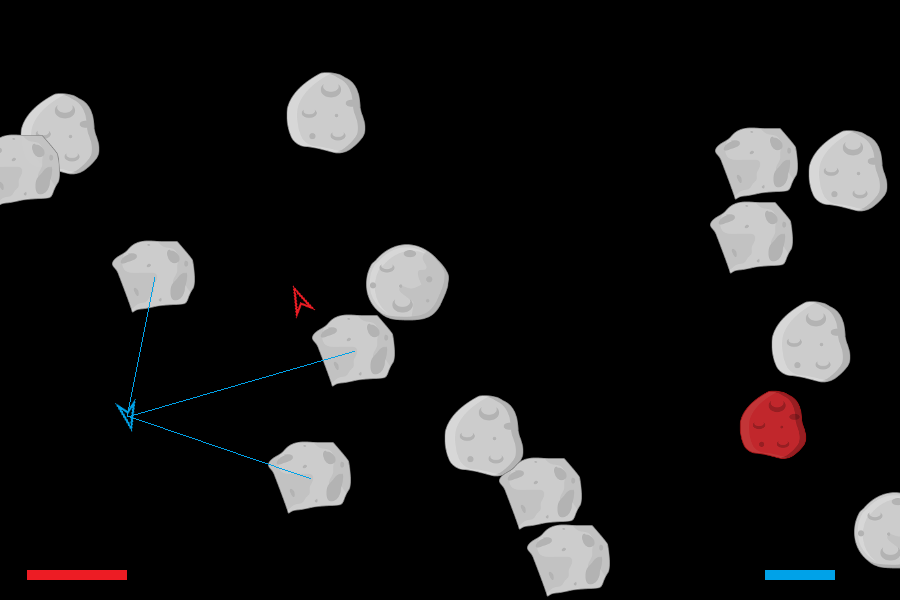
\includegraphics[width=150mm, height=100mm]{./Obrazky/N_nearest_asteroids.png}
\caption{Ukázka senzoru "N nejbližších asteroidů od vesmírné lodi" pro N=3}
\label{obr02:}
\end{figure}


\section{Akční plán}
Druhou zmíněnou abstrakcí jsou akční plány, jejich smyslem je, podobně jako u senzorů, namísto elementárních akcí nízké úrovně volit akční plány vyšší úrovně.
Akční plán představuje posloupnost množin elementárních akcí. Akční plány mají vždy nějaký cíl a záleží o jaký typ akčního plánu jde. 
Hlavní myšlenkou akčních plánů je, že využitím posloupnosti akcí, které aplikujeme během následujících krocích hry, můžeme dosáhnout komplexnějších důsledků, než kterých dosáhneme jednorázovým provedením libovolné elementární akce.
\par
Podobně jako u senzorických metod i zde hledání většiny akčních plánů probíhá simulací hry. Každý akční plán se snaží dosáhnout konkrétního cíle. V rámci simulace se 

\subsection{Jednotliv plány}
\begin{itemize}
    \item Útočný plán - V této simulace se hledá, jak se má vesmírná loď otočit a jakou střelu vystřelit, aby rozstřelila asteroid, kterým může zasáhnout nepřátelskou loď.
        Simulace postupně prochází všechny možné otočení a následné střely. Postupuje se inkrementálně. Vesmírná loď se v simulaci jednou otočí, vystřelí střelu a pokud střela zasáhne nějaký střední, nebo veliký asteroid. 
        Nad tímto asteroidem se následně zkouší, jestli vzniklé asteroidy rozstřelením zasáhnou nepřátelskou loď. Rozstřelení asteroidu se zkouší pro oba typy střel.
        \par
        V případě, že vystřelená střela nezasáhla žádný z asteroidů požadované velikosti, nebo rostřelené asteroidy nezasáhy cíl, se v simulaci vesmírná loď pokusí provést další rotaci a celý pokus o střelu opakovat.
        Pokud v simulaci nastalo úspěšné sestřelení, tak se vrací útočný akční plán, který obsahuje přílušný počet rotací následovaný střelou.
    
    \item Obranný plán - Pro hledání obraného plánu je nejprve potřeba vědět, před kterým asteroidem se chceme bránit. 
        A tomu právě využijeme připravené senzory. Obraný plán je vlastně složením dvou částí. První částí je rotace vesmírné lodi tak, aby mířila na asteroid, před kterým se chce bránit.
        A druhá část je samotná střelba, ta už není zcela součástí akčního plánu. Vyhodnocení, zda vystřelením střely sestřelíme konkrétní asteroid je opět záležitost jednoduché senzorické metody.
        \par
        Rotace vesmírné lodi, aby byla orientována směrem k danému asteroidu, není potřeba provádět simulací, stačí nám k tomu statický výpočet.
        Nejprve musíme zjistit, kde má ke srážce dojít. V případě, že vesmírná loď, anebo asteroid stojí staticky na místě, tak ke srážce dojde na současné poloze vesmírné lodi.
        Pokud jsou ale oba objekty v pohybu, tak ke srážce dojde na zcela jiném místě a toto musíme vzít v potaz.
        Pokud by se vesmírná loď otočila pouze vzhledem k současné poloze asteroidu, tak je možné, že by střelou mohla letící asteroid minout.
        Proto se namísto současné polohy asteroidu míří na cílovou polohu.
        Cílová poloha pro nás bude bod, který leží na přímce spojující tyto dva body a to ve vzdálenosti 15 procent jejich vzdálenosti blíže k polože asteroidu. 
        Tímto způsobem bude střela letět do směru letu asteroidu. Empiricky bylo vyzkoušeno, že toto funguje velmi dobře.
        Poté co určíme cílovou polohu, tak jen spočítáme rozdíl současného úhlu vesmírné lodi, od úhlu k cílové polože.
        Akční plán pak bude obsahovat potřebný počet rotací.       
    
    \item Úhybný plán - Jedná se také o defenzivní plán, ale místo přímé sestřelené nebezpečného asteroidu, se tento akční plán snaží asteroidu vyhnouot.
    Podobně jako u obranného plánu, potřebujeme vědět, jakému asteroidu se chceme vyhnout. Simulace postupně prochází všechny možné otočení a následnou akceleraci.
    Simulace akcelerace zkouší také inkrementálně počet potřebných akcelerací. Nejprve se vyzkouší provést akci akcelerace jednou a následně se simuluje pohyb vesmírné lodi a asteroidu.
    Pokud došlo ke srážce, tak se vyzkouší provést akci akcelerace dvakrát a opět se simuluje, zda se objekty srazí. 
    V případě úspěšného vyhnutí se vrátí úhybný plán obsahující akce rotace a následně potřebný počet akcí akcelerace.
    
    \item Zastavovací plán - Tento plán jsem vytvořil na základě sledování jak se chová úhybný plán. Úhybný plán vždy vrací nejkratší plán, který stačí na vyhnutí se srážce, proto většinou obsahuje minimálně počet rotací, který je dostačující.
        To má za následek, že agent, který se řídí pouze úhybními plány používá akceleraci mnohem častěji než rotace a lítá tak obrovskou rychlostí napříč prostorem. Proto mě napadlo, že by se mohl hodit akční plán, který vesmírnou loď uvede do klidu.
        \par
        Zastavovací plán má přímočarou myšlenku. 
        Nejdříve se vesmírná loď zrotuje, aby byla nasměrována proti směru pohybu a následně provede potřebný počet akcelerací, aby zpomalovala až do úplného zastavení. 
        Zastavovací plán ve výsledku obsahuje jistý počet akcí rotace následovaný potřebným počtem akcí akcelerace. 

        \par
        Tento akční plán mi připadal takový více lidský. V kombinaci s úhybným plánem se pak agent choval více přirozeně.
        Namísto zběsilého letu napříč prostorem se vesmírná loď po vyhnutí uvede do klidu.            
        
\end{itemize}


\subsection{Přepočítávání akčních plánů}
Získávání akčních plánů je výpočetně náročné, proto by bylo vhodné omezit jejich přepočítávání. Akční plány nám vracejí posloupnost akcí na více kroků dopředu a proto není potřeba je přepočítávat v každém kroku.
Změny mezi dvěmi po sobě jdoucími stavy hry není veliká, ale může být dostatečná na to, aby se přepočítaný plán lišil od předchozího.
V každém kroku hry se rozhoduje, zda se bude plán přepočítávat. Když je jednou plán vypočítaný, tak v dalších krocích stačí pouze vzít další akce z plánu a není potřeba žádného jiného výpočtu.
Plán se přepočítává, pokud uplynul daný počet pasivních kroků, ve kterých jsme pokračovali v již vytvořeném plánu, a nebo byl předchozí plán dokončen.
Počet neaktivních kroků se rovná konstaně \emph{\uppercase{inactive\_steps\_limit}}. 
S vyšším počtem pasivních kroků se velmi výrazně snižuje celkový čas odehrátí hry, ale počet kroků během hry se sníží jen minimálně (viz obr03).
Je zde vidět, že kvalita hráčů se mírně snižuje, ale v poměru kolik ušetříme času, je tato ztráta kvality zanedbatelná.
V pozdějších kapitolách se nám bude hodit odehrát velké množství her, proto si dovolíme nastavit vyšší počet pasivních kroků.


\begin{figure}[hp]

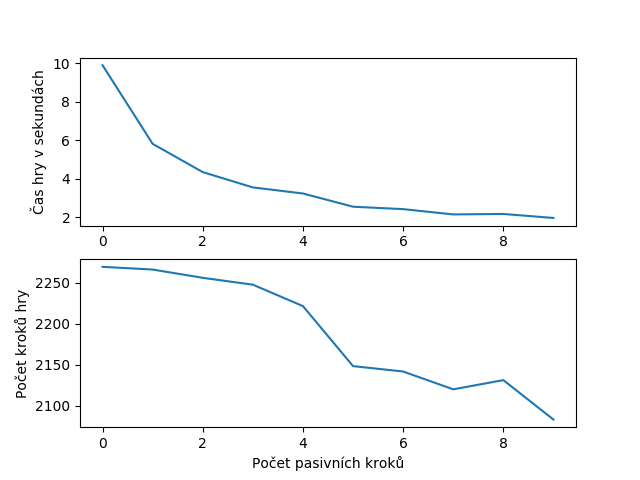
\includegraphics[width=150mm, height=120mm]{./Obrazky/Inactive_steps_comparison2.png}
\caption{Srovnání počtu neaktivních kroků k průměrné délce hry. Čísla byla získána průměrováním 40 her, kde proti sobě hráli agenti využívající pouze obranných plánů.}
\label{obr03:}
\end{figure}

\subsection{Použití akčních plánů}



